\subsection{Hardware}
\label{research:hardware}
The selection of hardware for usage in this product comes down to a combination of two vendors. Firstly the wireless adaptor manufacturer, such as Edimax, Netgear, Belkin, etc. that build the overall product. The decision of which manufacturer in this respect is not as important as the second, the chipset manufacturer.  These are companies such as Broadcom and Realtek, and this decision determines which operating systems are compatible, the device driver to use, and ultimately whether injection and monitoring are supported.

\subsubsection{Wireless Adaptor}
This boils down to device type, i.e. whether the adaptor is PCI, USB \nomenclature{USB}{Universal Serial Bus}, etc. and does not make any particular difference.
\subsubsection{Wireless Chipsets}
Consideration has to be taken into the chipset wireless adaptors use for compatibility with injection and monitoring libraries. Certain vendors, such as RealTek, support the open source community more-so than others which means drivers can be written for adaptors that use them.

Firstly I tried to use a wireless adaptor purchased for use with the Raspberry Pi.

\begin{figure}[h!]
\centering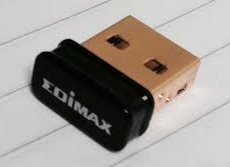
\includegraphics{research/figures/edimax.png}
\caption{Edimax EW-7811UN wireless adaptor.}
\end{figure}

The Edimax EW-7811UN fulfilled the first part of the criteria by using the RTL8188CUS chipset as working drivers were available for Linux; however, after initial tests against PyLorcon2 it was determined that the adaptor was not supported. Most likely due to it's newer chipset and Lorcon having not been updated in approximately two years. 

The second suggestion for a wireless adaptor to use with Lorcon was the Alfa AWUS036H, which came from various support forums that had users querying which adaptor to use with the Air-ng applications.  

\begin{figure}[h!]
\centering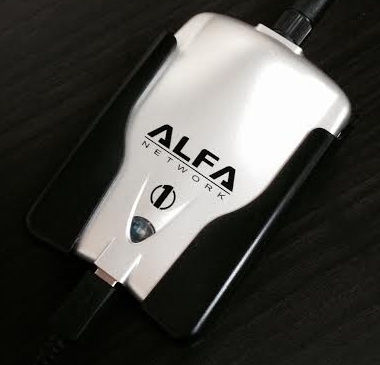
\includegraphics{research/figures/alfa.png}
\caption{Alfa AWUS036H wireless adaptor.}
\label{research:fig-alfa}
\end{figure}
\newpage
This is ideal as that suite of software will more than likely play a large role in the application's implementation as it is very good at specific tasks such as creating fake access points, and creating wireless monitor mode interfaces. The Alfa wireless adaptor is built upon the Realtek RTL8187 chipset, which, as noted above, is also beneficial due to RealTek's support toward the open source community.